% Options for packages loaded elsewhere
% Options for packages loaded elsewhere
\PassOptionsToPackage{unicode}{hyperref}
\PassOptionsToPackage{hyphens}{url}
\PassOptionsToPackage{dvipsnames,svgnames,x11names}{xcolor}
%
\documentclass[
  british,
  a4paper,
]{article}
\usepackage{xcolor}
\usepackage{amsmath,amssymb}
\setcounter{secnumdepth}{-\maxdimen} % remove section numbering
\usepackage{iftex}
\ifPDFTeX
  \usepackage[T1]{fontenc}
  \usepackage[utf8]{inputenc}
  \usepackage{textcomp} % provide euro and other symbols
\else % if luatex or xetex
  \usepackage{unicode-math} % this also loads fontspec
  \defaultfontfeatures{Scale=MatchLowercase}
  \defaultfontfeatures[\rmfamily]{Ligatures=TeX,Scale=1}
\fi
\usepackage{lmodern}
\ifPDFTeX\else
  % xetex/luatex font selection
\fi
% Use upquote if available, for straight quotes in verbatim environments
\IfFileExists{upquote.sty}{\usepackage{upquote}}{}
\IfFileExists{microtype.sty}{% use microtype if available
  \usepackage[]{microtype}
  \UseMicrotypeSet[protrusion]{basicmath} % disable protrusion for tt fonts
}{}
\makeatletter
\@ifundefined{KOMAClassName}{% if non-KOMA class
  \IfFileExists{parskip.sty}{%
    \usepackage{parskip}
  }{% else
    \setlength{\parindent}{0pt}
    \setlength{\parskip}{6pt plus 2pt minus 1pt}}
}{% if KOMA class
  \KOMAoptions{parskip=half}}
\makeatother
% Make \paragraph and \subparagraph free-standing
\makeatletter
\ifx\paragraph\undefined\else
  \let\oldparagraph\paragraph
  \renewcommand{\paragraph}{
    \@ifstar
      \xxxParagraphStar
      \xxxParagraphNoStar
  }
  \newcommand{\xxxParagraphStar}[1]{\oldparagraph*{#1}\mbox{}}
  \newcommand{\xxxParagraphNoStar}[1]{\oldparagraph{#1}\mbox{}}
\fi
\ifx\subparagraph\undefined\else
  \let\oldsubparagraph\subparagraph
  \renewcommand{\subparagraph}{
    \@ifstar
      \xxxSubParagraphStar
      \xxxSubParagraphNoStar
  }
  \newcommand{\xxxSubParagraphStar}[1]{\oldsubparagraph*{#1}\mbox{}}
  \newcommand{\xxxSubParagraphNoStar}[1]{\oldsubparagraph{#1}\mbox{}}
\fi
\makeatother


\usepackage{longtable,booktabs,array}
\newcounter{none} % for unnumbered tables
\usepackage{calc} % for calculating minipage widths
% Correct order of tables after \paragraph or \subparagraph
\usepackage{etoolbox}
\makeatletter
\patchcmd\longtable{\par}{\if@noskipsec\mbox{}\fi\par}{}{}
\makeatother
% Allow footnotes in longtable head/foot
\IfFileExists{footnotehyper.sty}{\usepackage{footnotehyper}}{\usepackage{footnote}}
\makesavenoteenv{longtable}
\usepackage{graphicx}
\makeatletter
\newsavebox\pandoc@box
\newcommand*\pandocbounded[1]{% scales image to fit in text height/width
  \sbox\pandoc@box{#1}%
  \Gscale@div\@tempa{\textheight}{\dimexpr\ht\pandoc@box+\dp\pandoc@box\relax}%
  \Gscale@div\@tempb{\linewidth}{\wd\pandoc@box}%
  \ifdim\@tempb\p@<\@tempa\p@\let\@tempa\@tempb\fi% select the smaller of both
  \ifdim\@tempa\p@<\p@\scalebox{\@tempa}{\usebox\pandoc@box}%
  \else\usebox{\pandoc@box}%
  \fi%
}
% Set default figure placement to htbp
\def\fps@figure{htbp}
\makeatother



\ifLuaTeX
\usepackage[bidi=basic,shorthands=off]{babel}
\else
\usepackage[bidi=default,shorthands=off]{babel}
\fi
\ifLuaTeX
  \usepackage{selnolig} % disable illegal ligatures
\fi


\setlength{\emergencystretch}{3em} % prevent overfull lines

\providecommand{\tightlist}{%
  \setlength{\itemsep}{0pt}\setlength{\parskip}{0pt}}



 


\makeatletter
\@ifpackageloaded{tcolorbox}{}{\usepackage[skins,breakable]{tcolorbox}}
\@ifpackageloaded{fontawesome5}{}{\usepackage{fontawesome5}}
\definecolor{quarto-callout-color}{HTML}{909090}
\definecolor{quarto-callout-note-color}{HTML}{0758E5}
\definecolor{quarto-callout-important-color}{HTML}{CC1914}
\definecolor{quarto-callout-warning-color}{HTML}{EB9113}
\definecolor{quarto-callout-tip-color}{HTML}{00A047}
\definecolor{quarto-callout-caution-color}{HTML}{FC5300}
\definecolor{quarto-callout-color-frame}{HTML}{acacac}
\definecolor{quarto-callout-note-color-frame}{HTML}{4582ec}
\definecolor{quarto-callout-important-color-frame}{HTML}{d9534f}
\definecolor{quarto-callout-warning-color-frame}{HTML}{f0ad4e}
\definecolor{quarto-callout-tip-color-frame}{HTML}{02b875}
\definecolor{quarto-callout-caution-color-frame}{HTML}{fd7e14}
\makeatother
\makeatletter
\@ifpackageloaded{caption}{}{\usepackage{caption}}
\AtBeginDocument{%
\ifdefined\contentsname
  \renewcommand*\contentsname{Table of contents}
\else
  \newcommand\contentsname{Table of contents}
\fi
\ifdefined\listfigurename
  \renewcommand*\listfigurename{List of Figures}
\else
  \newcommand\listfigurename{List of Figures}
\fi
\ifdefined\listtablename
  \renewcommand*\listtablename{List of Tables}
\else
  \newcommand\listtablename{List of Tables}
\fi
\ifdefined\figurename
  \renewcommand*\figurename{Figure}
\else
  \newcommand\figurename{Figure}
\fi
\ifdefined\tablename
  \renewcommand*\tablename{Table}
\else
  \newcommand\tablename{Table}
\fi
}
\@ifpackageloaded{float}{}{\usepackage{float}}
\floatstyle{ruled}
\@ifundefined{c@chapter}{\newfloat{codelisting}{h}{lop}}{\newfloat{codelisting}{h}{lop}[chapter]}
\floatname{codelisting}{Listing}
\newcommand*\listoflistings{\listof{codelisting}{List of Listings}}
\makeatother
\makeatletter
\makeatother
\makeatletter
\@ifpackageloaded{caption}{}{\usepackage{caption}}
\@ifpackageloaded{subcaption}{}{\usepackage{subcaption}}
\makeatother
\usepackage{bookmark}
\IfFileExists{xurl.sty}{\usepackage{xurl}}{} % add URL line breaks if available
\urlstyle{same}
% fallback for those not using the hyperref driver hyperxmp:
\makeatletter
\@ifundefined{xmpquote}{\newcommand{\xmpquote}[1]{#1}}{}
\makeatother
\hypersetup{
  pdftitle={What drives industrial output in five emerging economies},
  pdfauthor={Carlos Galindo},
  pdflang={en-GB},
  colorlinks=true,
  linkcolor={blue},
  filecolor={Maroon},
  citecolor={Blue},
  urlcolor={Blue},
  pdfcreator={LaTeX via pandoc}}


\title{What drives industrial output in five emerging economies}
\usepackage{etoolbox}
\makeatletter
\providecommand{\subtitle}[1]{% add subtitle to \maketitle
  \apptocmd{\@title}{\par {\large #1 \par}}{}{}
}
\makeatother
\subtitle{Across 27 years of monthly data, global risk appetite is the
one robust driver; policy rates show no measurable direct effect.}
\author{Carlos Galindo}
\date{}
\begin{document}
\maketitle


\begin{tcolorbox}[enhanced jigsaw, arc=.35mm, bottomrule=.15mm, breakable, colback=white, colframe=quarto-callout-note-color-frame, left=2mm, leftrule=.75mm, opacityback=0, rightrule=.15mm, toprule=.15mm]

\vspace{-3mm}\textbf{At a glance}\vspace{3mm}

\begin{itemize}
\tightlist
\item
  \textbf{Question.} What moves industrial output growth in a small set
  of open emerging economies: domestic monetary policy, or conditions
  set abroad?
\item
  \textbf{Approach.} A dynamic panel of five economies, monthly from
  1999 to 2026, estimated by several methods that treat persistence and
  endogeneity differently.
\item
  \textbf{Finding.} Output growth is highly persistent. Global risk
  appetite is the one driver that survives every specification. The
  policy rate has no measurable direct effect.
\item
  \textbf{Why it matters.} For a forecaster or a policymaker, it shifts
  attention from the domestic rate path to the global risk regime, and
  it shows how fragile a ``significant'' policy effect can be.
\end{itemize}

\end{tcolorbox}

\subsection{The question}\label{the-question}

Emerging-economy industrial output is often modelled as a response to
domestic conditions: the policy rate, inflation, the exchange rate. Yet
these economies are small, open and exposed to the same global swings in
risk appetite, commodity prices and financing conditions. A model that
includes only domestic variables can attribute to home policy what
really belongs to the world.

The project asks a plain question: once persistence is accounted for,
which variables have a stable, measurable association with industrial
output growth across five emerging economies? The obvious approach, a
single regression on one country, falls short for three reasons. A
single country offers too little variation to separate global from local
forces. Output growth is strongly autocorrelated, which biases naive
estimates. And policy rates respond to the same conditions they are
supposed to influence, so a simple regression mixes cause and effect.

\subsection{Approach}\label{approach}

\textbf{Data.} The panel covers five emerging economies at monthly
frequency from January 1999 to February 2026, a balanced panel of about
326 months per economy, or 1,630 country-months before lags. The outcome
is the year-on-year growth rate of industrial production. The
explanatory variables are the policy rate, domestic inflation, changes
in sovereign spreads and the oil price in the main specification, with a
second specification on the monetary channel using the real interest
rate, the change in the real effective exchange rate and a measure of
global equity-market volatility. Daily and weekly series were averaged
to monthly rather than sampled at month end, which matters in crisis
months when volatility is extreme.

\textbf{Method.} The core model is a dynamic panel: output growth
depends on its own lag plus the drivers above. It was estimated several
ways, so that no conclusion depends on a single estimator:

\begin{itemize}
\tightlist
\item
  pooled least squares, which ignores country differences;
\item
  fixed effects, with standard errors that allow for correlation across
  countries within the same month;
\item
  feasible generalised least squares;
\item
  two instrumental-variable estimators that use lagged levels of output
  growth to handle the endogeneity that lagged outcomes create.
\end{itemize}

\textbf{Checks.} With only five economies and a long time dimension, the
usual dynamic-panel worry runs the other way. The classic small-sample
bias in fixed effects is of order one over T, roughly 0.003 here, so
fixed effects is reliable. By contrast, estimators designed for many
units and few periods can generate far more moment conditions than there
are cross-sections. An earlier estimation with a very large instrument
set produced a pathological over-identification test and a spurious
significant policy-rate coefficient. Using a small, pooled instrument
set restored a test that does not reject. Results were also re-estimated
after correcting one economy's inflation series, which removed a
spurious significance in the real rate and strengthened the global-risk
effect.

\subsection{What the work shows}\label{what-the-work-shows}

\textbf{Persistence dominates.} The coefficient on lagged output growth
is about 0.84 under fixed effects, close to the pooled value, and 0.67
to 0.70 under the instrumental-variable estimators. That ordering is
what theory predicts: pooled estimation overstates persistence, and the
instrumented estimates sit lower. At 0.84 a shock to output growth has a
half-life of roughly four months. Most of the explained variation, about
71 per cent in the levels models, comes from this inertia.

\textbf{Global risk appetite is the one robust driver.} In the
monetary-channel specification the coefficient on global equity-market
volatility is about −0.09 under fixed effects and −0.10 under
instrumental variables, and it is significant at the one per cent level
in both. A one-point rise in the volatility measure lowers output growth
by about a tenth of a percentage point in the same month. Because of
persistence, the cumulative cost of a one-off 20-point surge is roughly
10 percentage points of output growth spread over the decay path, with
about 1.9 points on impact. That is the scale of episodes such as the
global financial crisis and the pandemic.

\textbf{No measurable direct effect of the policy rate.} In the main
specification the policy-rate coefficient is −0.014 with a robust
standard error of 0.076 under fixed effects, and +0.190 with a standard
error of 0.341 under the GMM instrumental-variable estimator. Neither is
distinguishable from zero, and the sign changes. The real rate gives the
same answer. Two forces plausibly offset: higher rates restrain
activity, while central banks raise rates when activity is strong. The
work does not claim policy is irrelevant. It claims that a direct,
contemporaneous effect cannot be measured in this panel once global
conditions are controlled.

\begin{figure}

\centering{

\pandocbounded{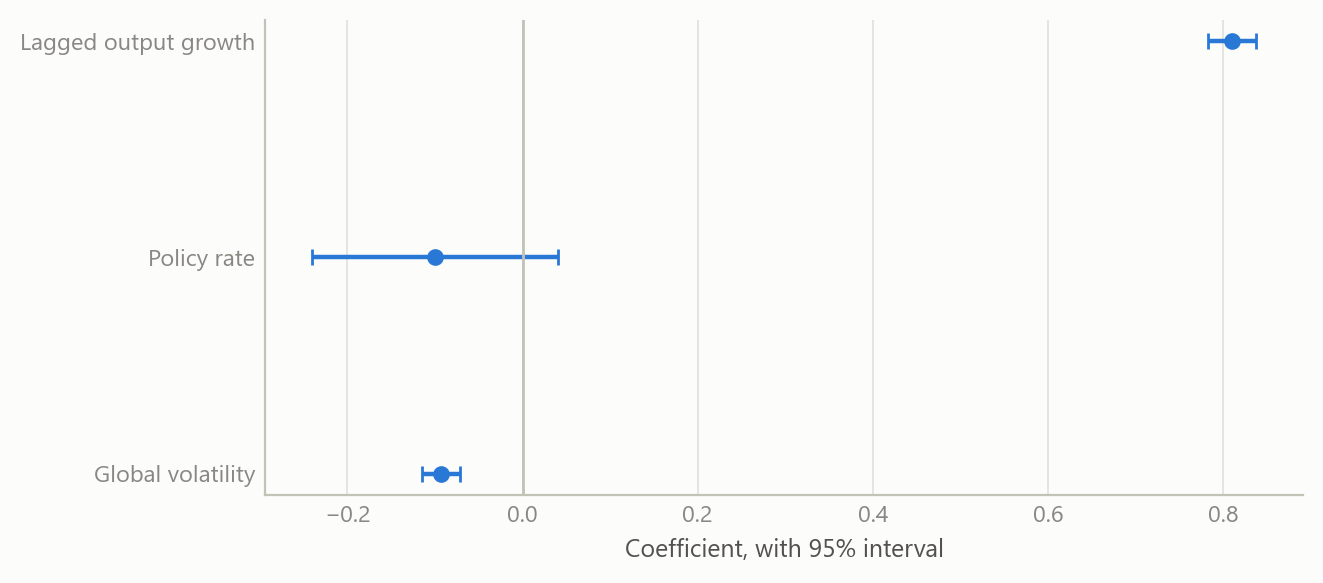
\includegraphics[keepaspectratio]{index_files/figure-latex/fig-coef-output-1.png}}

}

\caption{\label{fig-coef}Estimated effects in a simulated panel built to
mimic the study's structure (five units, 326 months): persistence and
global risk appetite are recovered, the policy rate is not
distinguishable from zero (simulated data).}

\end{figure}%

\textbf{The other channels are weak or conditional.} Inflation has a
negative sign in every specification, consistent with a cost channel,
but it is significant only at the ten per cent level and loses
significance once errors are clustered by month. Oil is insignificant in
levels but positive in first differences, which reads as a global-demand
proxy rather than a supply shock for these economies. Sovereign-spread
changes have no contemporaneous effect; the work suggests that any
effect runs through longer lags, spread levels or thresholds, and treats
that as untested.

\begin{figure}

\centering{

\pandocbounded{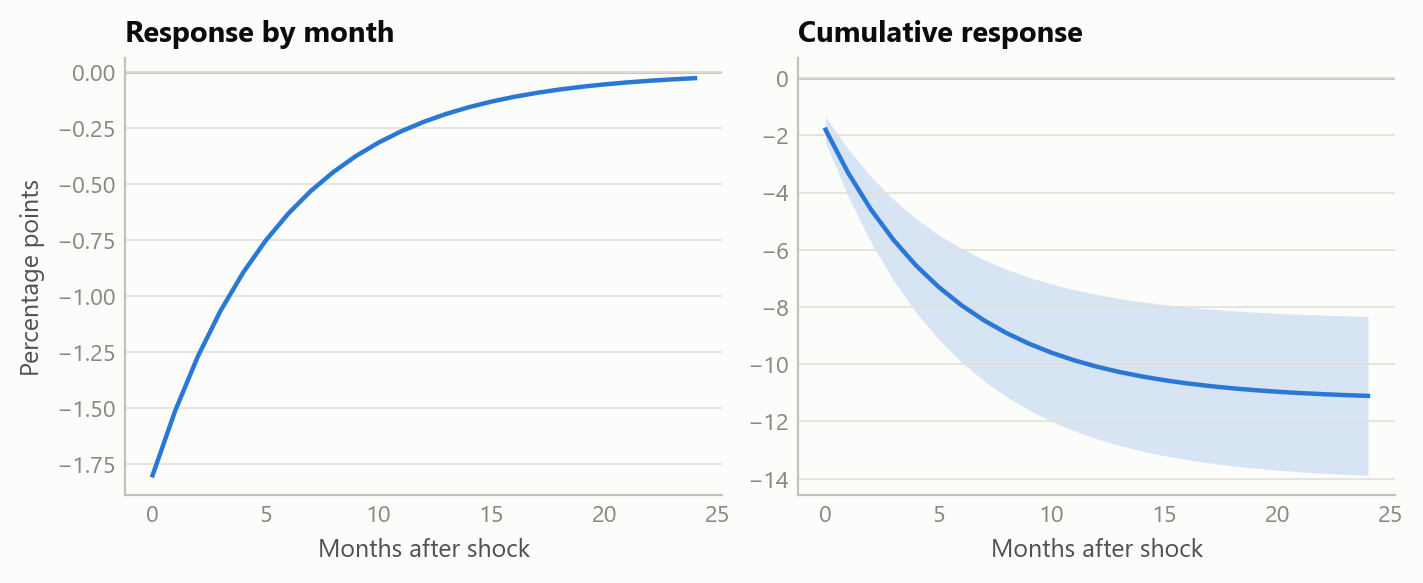
\includegraphics[keepaspectratio]{index_files/figure-latex/fig-irf-output-1.png}}

}

\caption{\label{fig-irf}Cumulative response of output growth to a
one-off 20-point rise in global volatility, from a simulated persistent
process with the same structure (simulated data).}

\end{figure}%

\subsection{Insights}\label{insights}

\begin{enumerate}
\def\labelenumi{\arabic{enumi}.}
\tightlist
\item
  \textbf{Look abroad first.} In small open economies the global risk
  regime explains more output variation than any domestic variable
  tested.
\item
  \textbf{A null is a result.} The absence of a direct policy effect
  holds across estimators once the instrument set is credible, and an
  earlier ``significant'' effect did not.
\item
  \textbf{Match the estimator to the panel.} With few units and many
  periods, fixed effects is sound and heavily instrumented GMM is the
  hazard, the reverse of the textbook case.
\item
  \textbf{Persistence amplifies.} A small contemporaneous effect becomes
  a large cumulative one when output growth has a four-month half-life.
\item
  \textbf{Data validation can change conclusions.} Correcting one
  country's series moved three of the headline coefficients.
\end{enumerate}

\subsection{Limits and next steps}\label{limits-and-next-steps}

The panel has only five economies, so cross-country inference is limited
and the results describe this group, not emerging markets in general.
Monthly industrial output is a narrow measure of activity. The
policy-rate result is a statement about a direct, linear,
contemporaneous effect; it says nothing about expectations, forward
guidance or effects at longer lags. The exclusion restrictions behind
the instrumental-variable estimates cannot be proven, only tested for
consistency, and with a small set of instruments the over-identification
test has little power. Next steps are distributed-lag and threshold
versions of the spread channel, a larger panel, and separating pre- and
post-crisis samples.

\subsection{About the evidence}\label{about-the-evidence}

The study is real work on public macroeconomic and market series,
covering 1999 to early 2026, carried out in an AI-assisted workflow
during 2025 and 2026. The figures here are illustrative: they use
simulated data with the same number of units, frequency and persistence,
and they show the method, not the results.

Figures and tables marked \emph{simulated} are generated from simulated
data built to share the structure of the analysis (its variables,
horizons and frequencies). They show how the method works and what its
output looks like; they are not the project's results. Results stated in
the text are the project's own. Methods are described at the level of a
methods section. Code and data pipelines are not reproduced here.




\end{document}
